\documentclass[a4paper]{article}

\usepackage[utf8]{inputenc}
\usepackage[T1]{fontenc}
\usepackage[italian]{babel}

\usepackage{graphicx}
\usepackage{siunitx}

\newcommand*\de{\mathrm{d}}

\begin{document}

\marginpar{punto 1}

Scegliamo di usare, in ordine dal basso verso l'alto, i PMT 2, 3, 4.

\marginpar{punto 2}

Accendiamo il PMT~2 a \SI{1500}V.

\marginpar{punto 3}

Schizzo dei segnali del PMT visti sull'oscilloscopio:

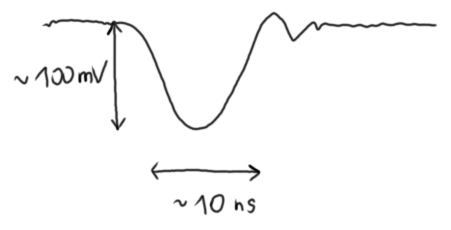
\includegraphics[width=9cm]{fig3a}

Con il trigger a \SI{-27}{mV}, contando a mano su \SI1{min}, otteniamo $\sim\SI1{Hz}$.

\paragraph{Amplificazione}

Stimiamo l'energia rilasciata da una particella nello scintillatore.
Supponiamo MIP, quindi
$\de E/\rho\de x=\SI{1.5}{MeV\,g^{-1}\,cm^2}$.
Lo spessore dello scintillatore è $\sim\SI1\cm$ e la densità $\sim\SI1{g\,cm^{-3}}$,
quindi rilascia $\SI{1.5}{MeV} = \SI{2.4e-13}{J}$.

Stimiamo l'energia del segnale in uscita. È
$\int\de t\, I\cdot V \approx \Delta t\cdot V^2/R$
dove $R=\SI{50}\ohm$, quindi otteniamo
$\num{10e-9}\cdot(\num{100e-3})^2/50=\SI{2e-12}{J}$.

L'amplificazione complessiva è quindi $\sim10$, a naso ce la aspettavamo più grande.

\paragraph{Dipendenza rate dall'alimentazione}

Impostiamo la tensione di alimentazione a \SI{1600}V.
La frequenza di segnali aumenta notevolmente,
per contarli a mano alziamo\footnote{Trattando la logica negativa, useremo alto-basso riferito al modulo e spesso tralasceremo il segno $-$,  la strumentazione suggerisce questo approccio perché la vite della soglia del discriminatore aumenta (abbassa) la soglia in verso orario.} il trigger a \SI{150}{mV},
otteniamo $85/\SI1{min}$.

Con \SI{1800}V otteniamo $\sim\SI{100}{Hz}$ e con \SI{2000}V $\sim\SI{1}{kHz}$
(frequenze misurate dall'oscilloscopio).

\marginpar{punto 4}

\paragraph{Documentazione discriminatore}

Non troviamo la documentazione del nostro discriminatore tra quella fornita;
poiché è a 4 canali e l'unica documentazione per uno a quattro canali è il CAEN~N84,
e inoltre a parte colore e etichette appare identico,
leggiamo la documentazione per quello e chiameremo il nostro <<N84>>.

Documentazione:
ritardo \SI{14}{ns},
durata 6--400\,\si{ns},
soglia massima \SI{400}{mV}.

\paragraph{Verifica discriminatore}

Montiamo questo circuito:

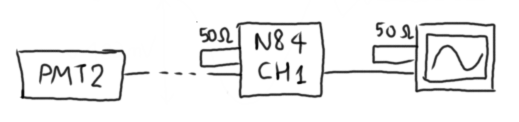
\includegraphics[width=9cm]{fig4a}

Girando la vite della durata vediamo che l'intervallo impostabile è circa 40--300\si{\,ns}.
È di tipo ``restarting'' perché per soglia abbastanza bassa si vedono durate doppie in uscita,
con soglia a opportuni valori intermedi si vedono alternativamente durate doppie oppure due singole, ravvicinate ma non più di tanto.
L'ampiezza è \SI{750}{mV} come atteso.
Verifichiamo la durata impostabile anche per il canale~2, è la stessa.

Modifichiamo il circuito in modo da visualizzare sia l'ingresso che l'uscita del discriminatore:

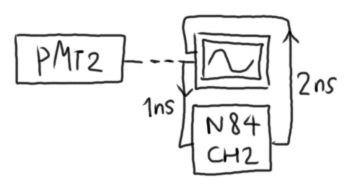
\includegraphics[width=5cm]{fig4b}

Misuriamo la soglia del discriminatore con l'oscilloscopio in questo modo:
triggeriamo sull'ingresso del discriminatore,
se la soglia del discriminatore è minore di quella del trigger
si vede sempre l'uscita del discriminatore,
viceversa a volte scompare.
Trovando due soglie del trigger più vicini possibili in modo che con una a volte scompare l'uscita (verificato su un tempo abbastanza lungo rispetto alla differenza delle soglie) e con l'altra no, si ottiene una misura della soglia del discriminatore.
Il problema di questa procedura è che il trigger dell'oscilloscopio funziona in modo diverso dal discriminatore, quindi non è detto che a parità di soglia vengano selezionati gli stessi segnali.
Con la soglia del discriminatore al massimo otteniamo le soglie del trigger 368 e \SI{376}{mV},
mentre il TP del discriminatore segna \SI{0.411}V, quindi lo scarto è circa \SI8\percent.

\end{document}
